
% ****************** Diaporama ******************
\documentclass{beamer}


% ****************** Packages ******************
\usepackage[french]{babel}
\usepackage[T1]{fontenc}
\usepackage[utf8]{inputenc}
\usepackage{tikz}

\usetheme{Warsaw}


% **** logo de l'upmc ****
\logo{
\includegraphics[width=2cm]{images/logo_upmc.png}}

\addtobeamertemplate{footline}{\insertframenumber/\inserttotalframenumber}

% ****************** Info pour page de garde ******************
\title{iBalezator}

\author{Adrien Ferreira, Alexandra Hospital}

\institute{PSAR - UPMC}

\date{26 mars 2015}



% ****************** Page de garde ******************
\begin{document}

   \begin{frame}

      \titlepage

   \end{frame}


% ******************** Table des matieres ********************
%  S'ajoute à chaque fin de section pour montrer 
%  où on est dans la présensation 

\AtBeginSection[]
{
\begin{frame}

     \frametitle{Sommaire}

        \tableofcontents[currentsection]

\end{frame} 
}


% ************ Présentation du projet ************ 

\section{Présentation du projet}

	% *** Balezator en ligne ***
	\subsection{Balezator en ligne}

	\begin{frame}

		\frametitle{Lecture sur le manche}
			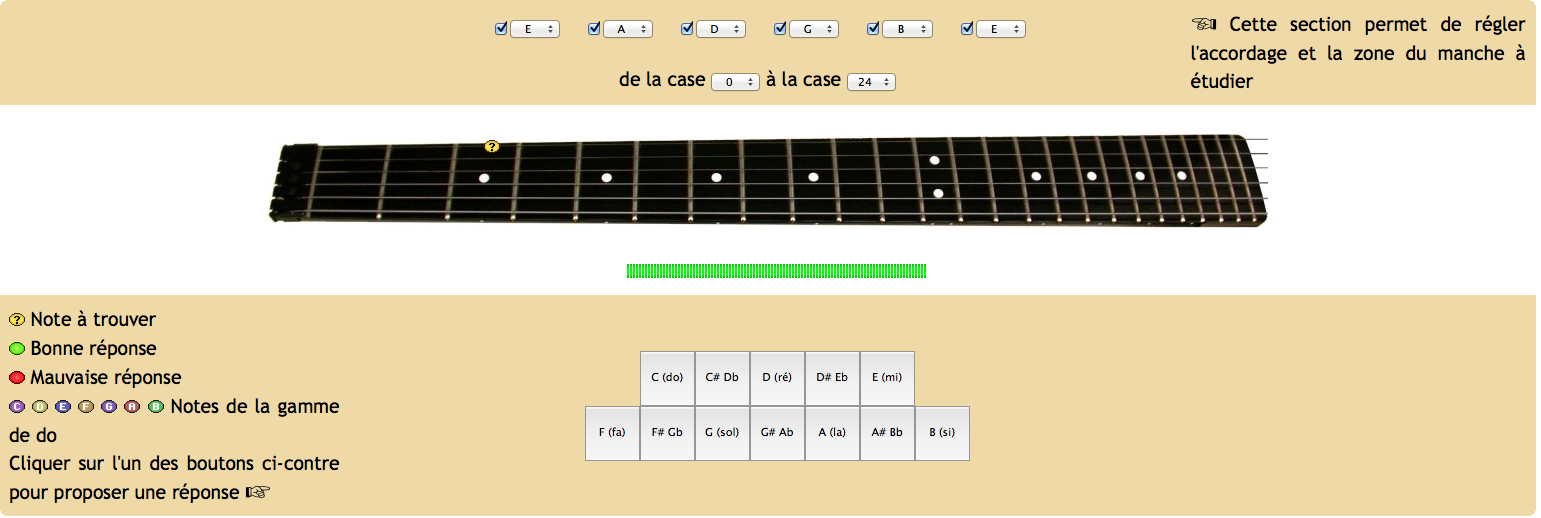
\includegraphics[width=10.5cm]{images/balezator_manche.png}
	\end{frame}

	\begin{frame}

		\frametitle{Lecture sur la portée}
			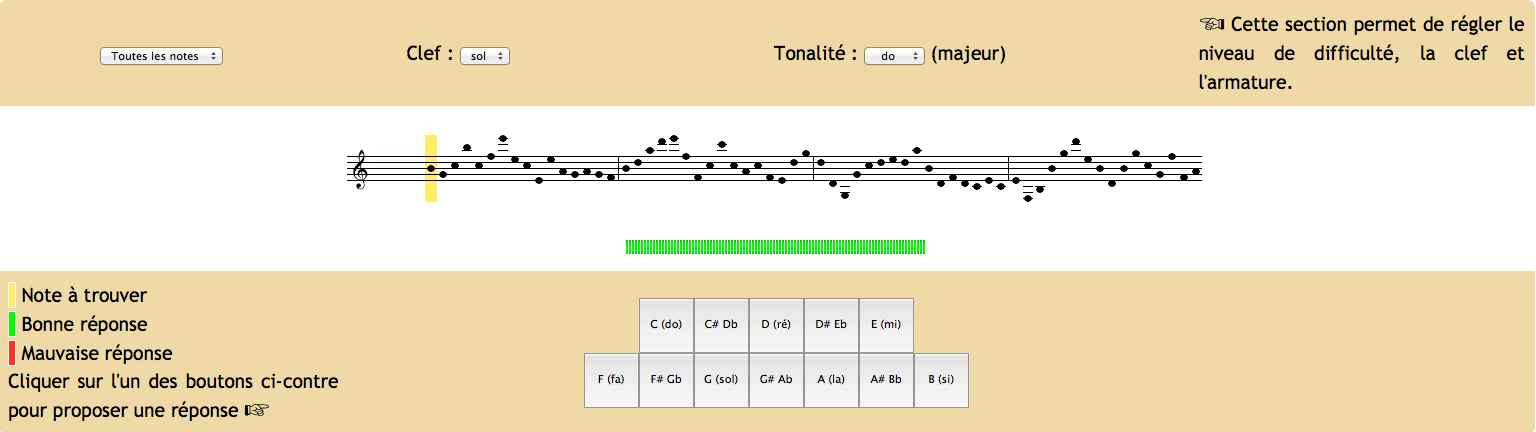
\includegraphics[width=10.5cm]{images/balezator_portee.png}

	\end{frame}



	% *** iBalezator ***
	\subsection{iBalezator}

	\begin{frame}
		\frametitle{Mode manche/clavier}
			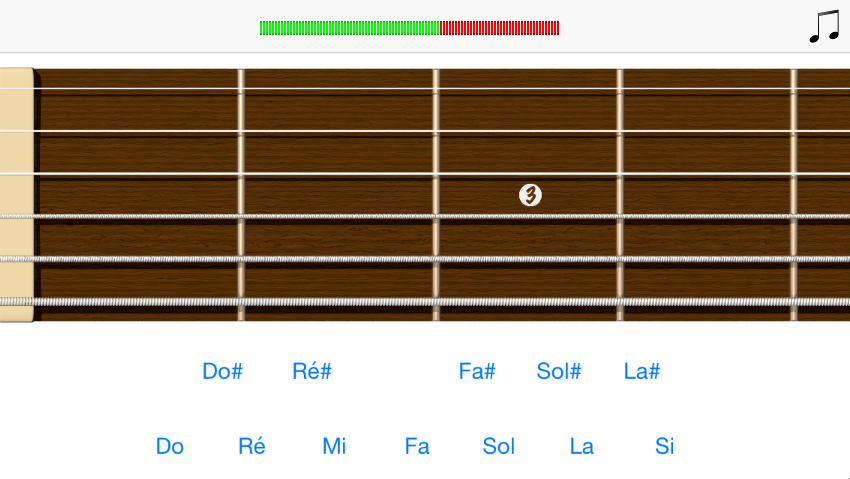
\includegraphics[width=10cm]{images/clavier_vierge.png}
	\end{frame}

	\begin{frame}
		\frametitle{Mode portée/manche}
			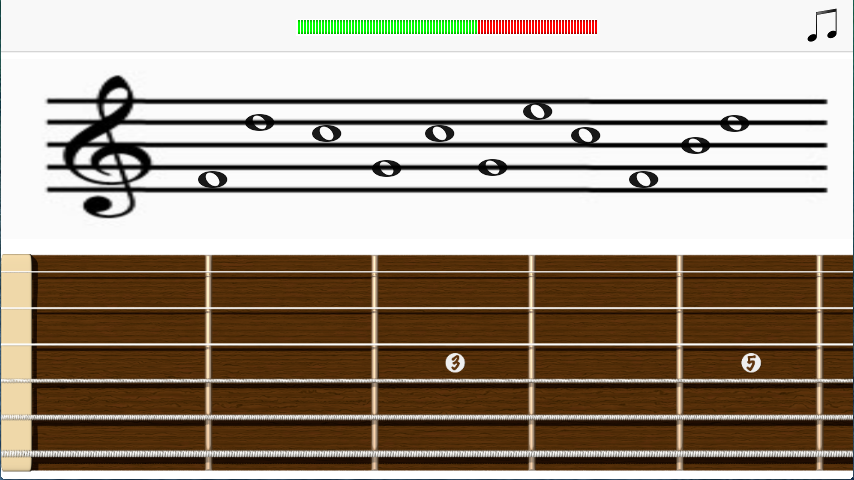
\includegraphics[width=10cm]{images/portee_vierge.png}
 
	\end{frame}


\section{Cahier des charges}

\begin{frame}
	\frametitle{Modifications}

	\begin{itemize}
		\item Veille concurrentielle 	
		\item Tests de validation : scénarios d'utilisation
	\end{itemize}
\end{frame}


% ******************* Scénarios Manche/clavier *******************
	\subsection{Scénarios manche/clavier}

	\begin{frame}

   		\frametitle{Manche/clavier}

       		\framesubtitle{Scénario 1}

		\begin{columns}

			 \begin{column}{0.33\textwidth}

				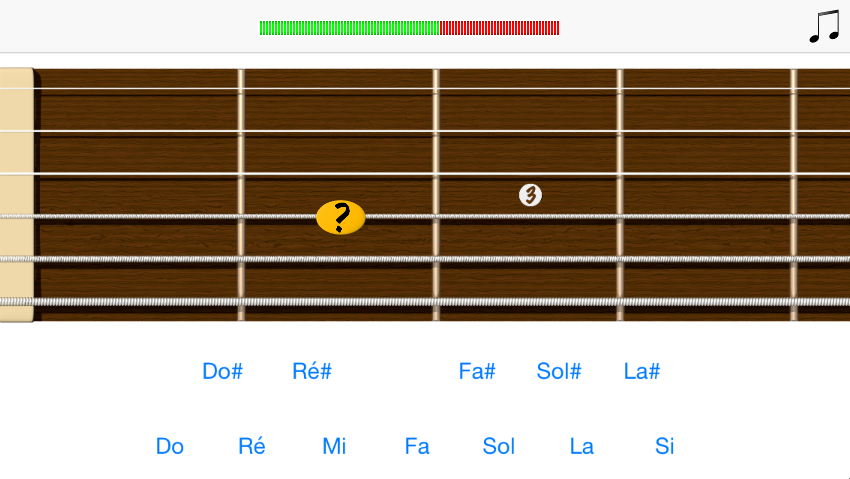
\includegraphics[width=3.5cm]{images/clavier_question.png}

			\end{column}

			 \begin{column}{0.33\textwidth}

				
			\end{column}

			 \begin{column}{0.33\textwidth}

				
			\end{column}

		\end{columns} 

	\end{frame}

	\begin{frame}

   		\frametitle{Manche/clavier}

       		\framesubtitle{Scénario 1}

		\begin{columns}

			 \begin{column}{0.33\textwidth}

				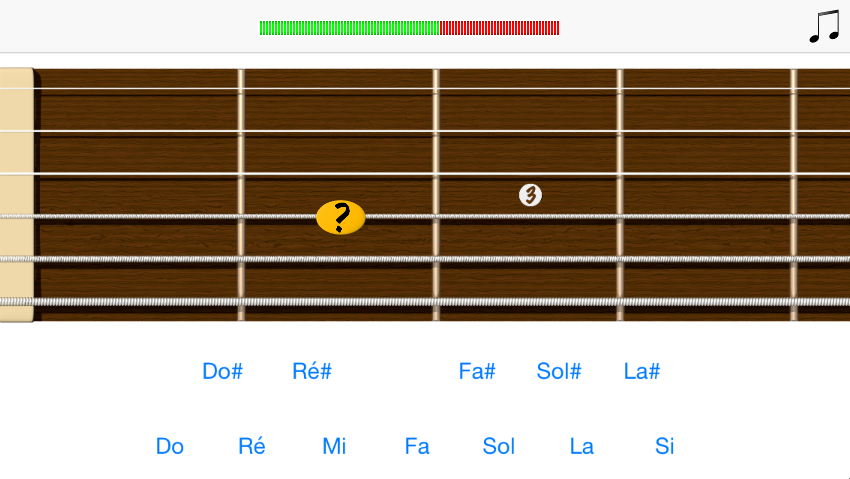
\includegraphics[width=3.5cm]{images/clavier_question.png}

			\end{column}

			 \begin{column}{0.33\textwidth}

				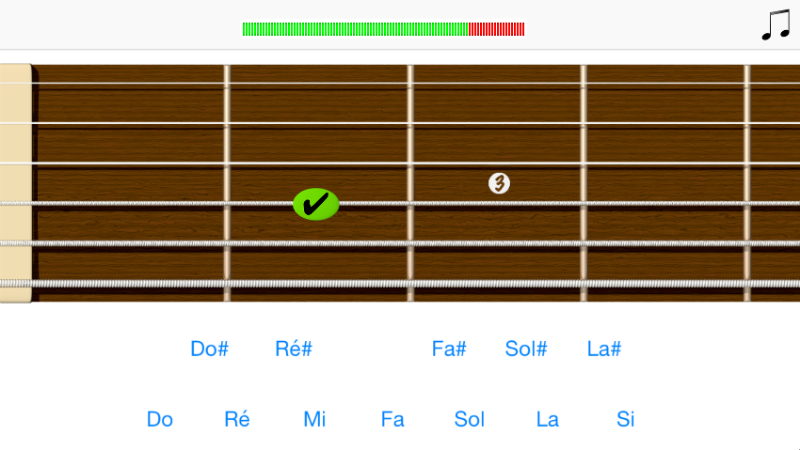
\includegraphics[width=3.5cm]{images/clavier_bonne.png}

				
			\end{column}

			 \begin{column}{0.33\textwidth}

				
			\end{column}

		\end{columns} 

	\end{frame}


	\begin{frame}

   		\frametitle{Manche/clavier}

       		\framesubtitle{Scénario 1}

	\begin{columns}

	 	\begin{column}{0.33\textwidth}

		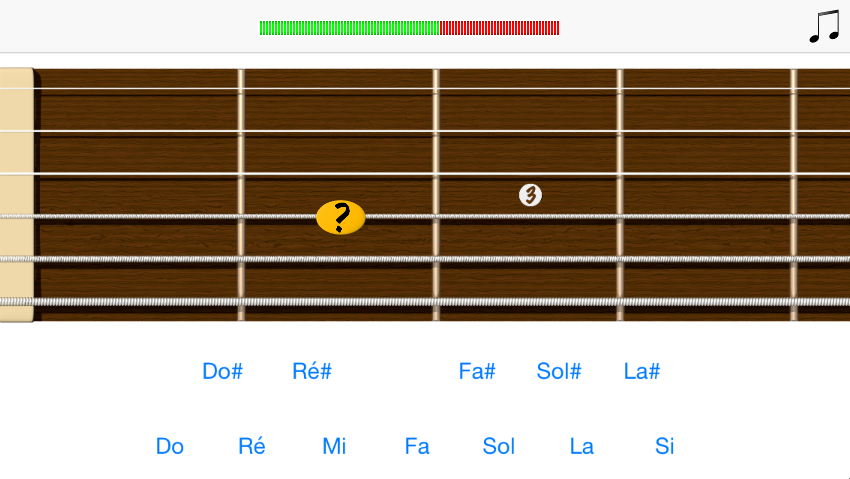
\includegraphics[width=3.5cm]{images/clavier_question.png}

		\end{column}

	 \begin{column}{0.33\textwidth}

		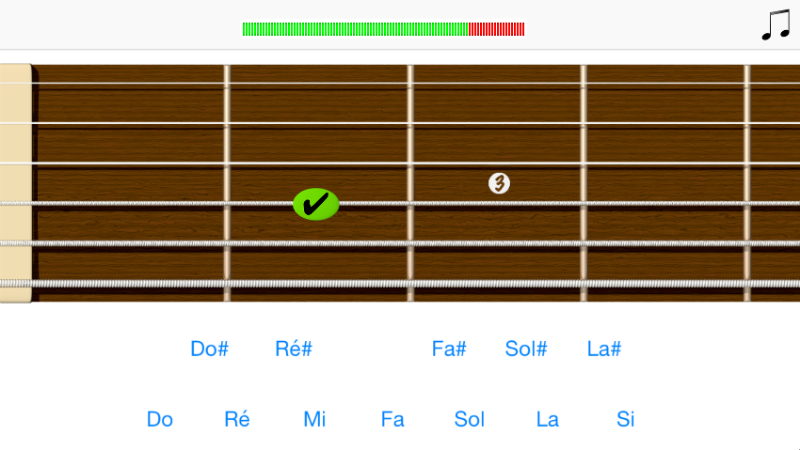
\includegraphics[width=3.5cm]{images/clavier_bonne.png}

	\end{column}

	 \begin{column}{0.33\textwidth}

		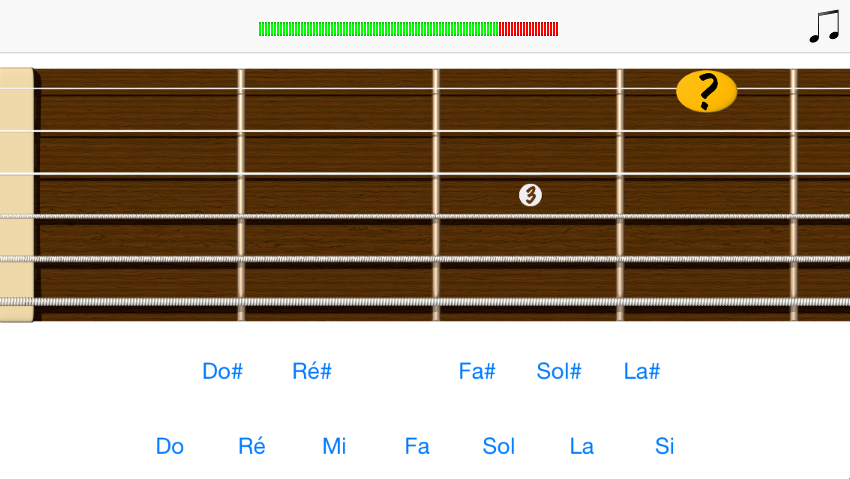
\includegraphics[width=3.5cm]{images/clavier_bonne_reponse_nouvelle_question.png}

	\end{column}

	\end{columns} 

	\end{frame}



				% ******* Scénario 2 *******


	\begin{frame}

   		\frametitle{Manche/clavier}

       		\framesubtitle{Scénario 2}

		\begin{columns}

			 \begin{column}{0.33\textwidth}

				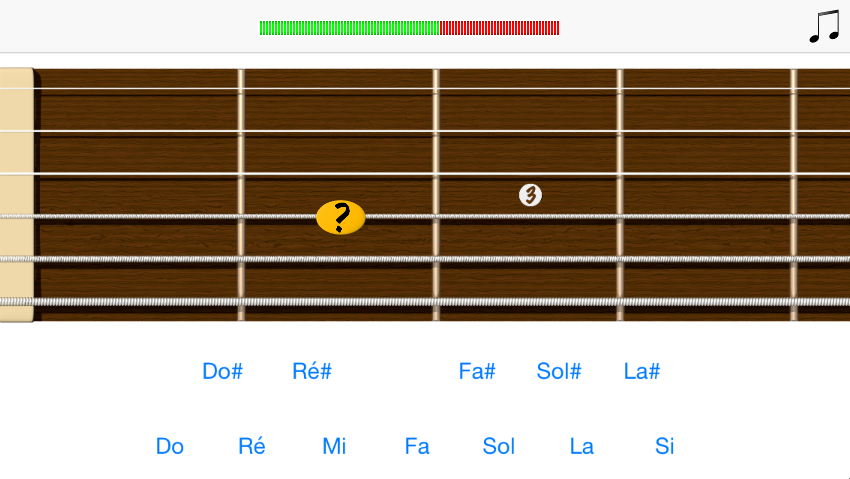
\includegraphics[width=3.5cm]{images/clavier_question.png}

			\end{column}

			 \begin{column}{0.33\textwidth}

				
			\end{column}

			 \begin{column}{0.33\textwidth}

				
			\end{column}

		\end{columns} 

	\end{frame}

	\begin{frame}

   		\frametitle{Manche/clavier}

       		\framesubtitle{Scénario 2}

		\begin{columns}

			 \begin{column}{0.33\textwidth}

				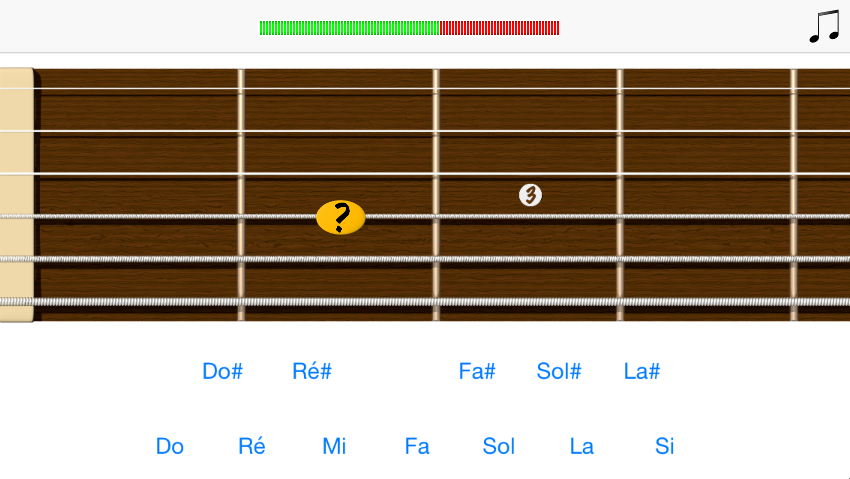
\includegraphics[width=3.5cm]{images/clavier_question.png}

			\end{column}

			 \begin{column}{0.33\textwidth}

				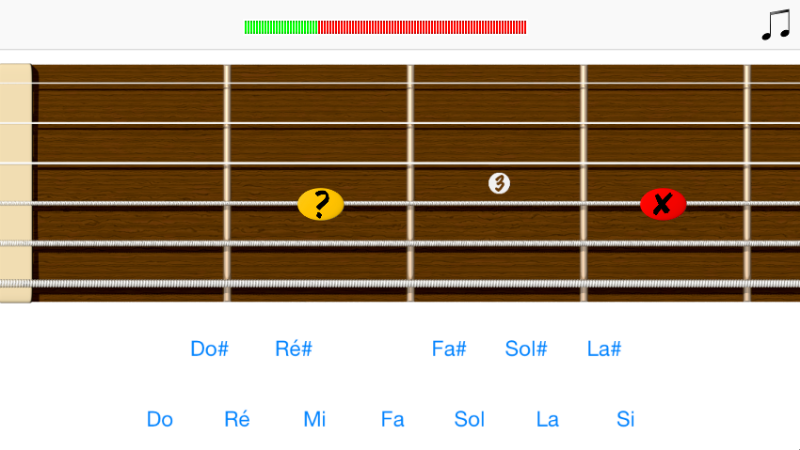
\includegraphics[width=3.5cm]{images/clavier_mauvaise.png}

				
			\end{column}

			 \begin{column}{0.33\textwidth}

				
			\end{column}

		\end{columns} 

	\end{frame}


	\begin{frame}

   		\frametitle{Manche/clavier}

       		\framesubtitle{Scénario 2}

	\begin{columns}

	 	\begin{column}{0.33\textwidth}

		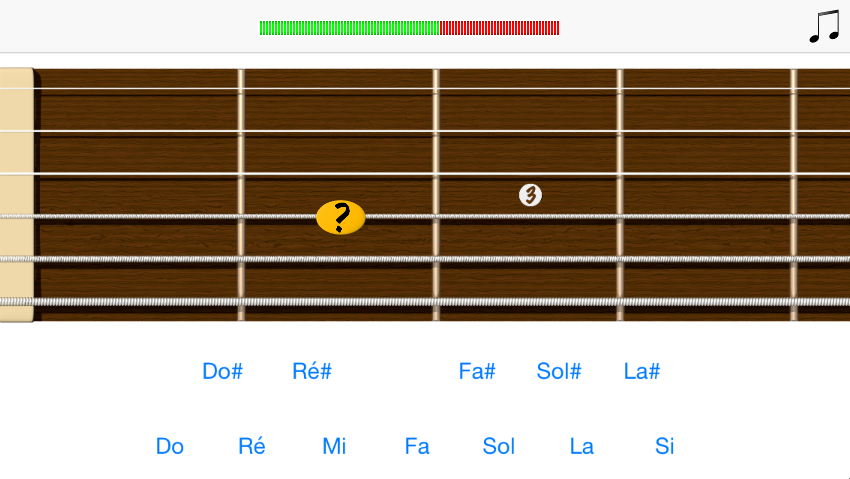
\includegraphics[width=3.5cm]{images/clavier_question.png}

		\end{column}

	 \begin{column}{0.33\textwidth}

		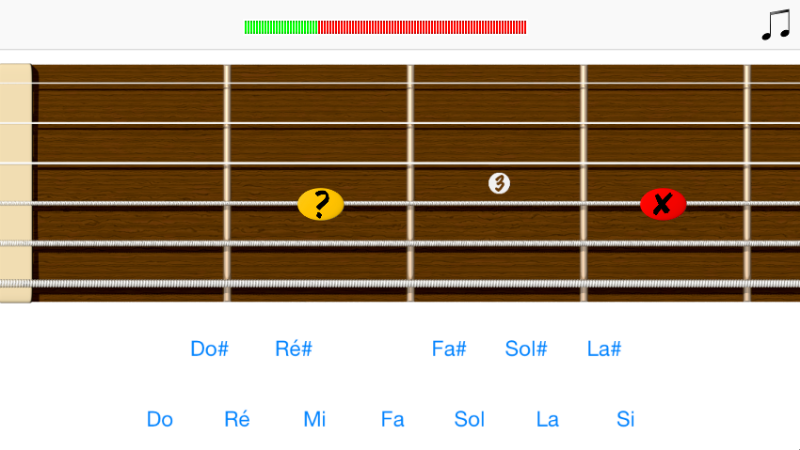
\includegraphics[width=3.5cm]{images/clavier_mauvaise.png}

	\end{column}

	 \begin{column}{0.33\textwidth}

		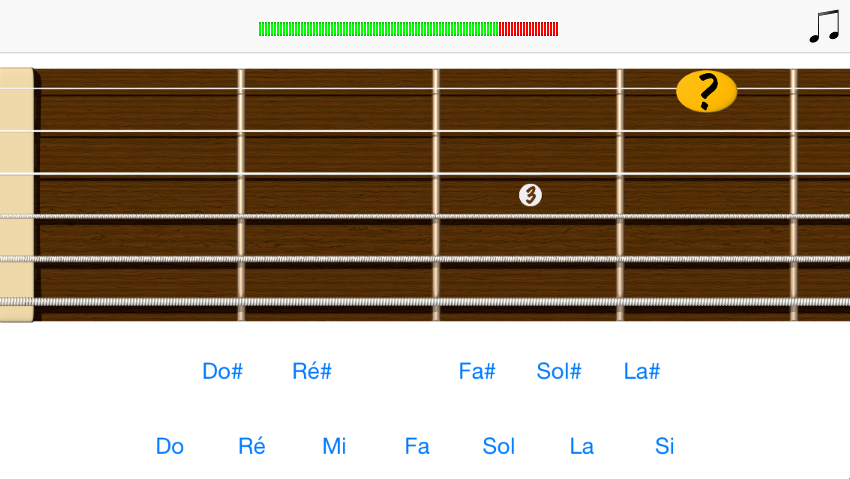
\includegraphics[width=3.5cm]{images/clavier_bonne_reponse_nouvelle_question.png}

	\end{column}

	\end{columns} 

	\end{frame}


				%****** Scénario 3 ******%


	\begin{frame}

   		\frametitle{Manche/clavier}

       		\framesubtitle{Scénario 3}

		\begin{columns}

			 \begin{column}{0.4\textwidth}

				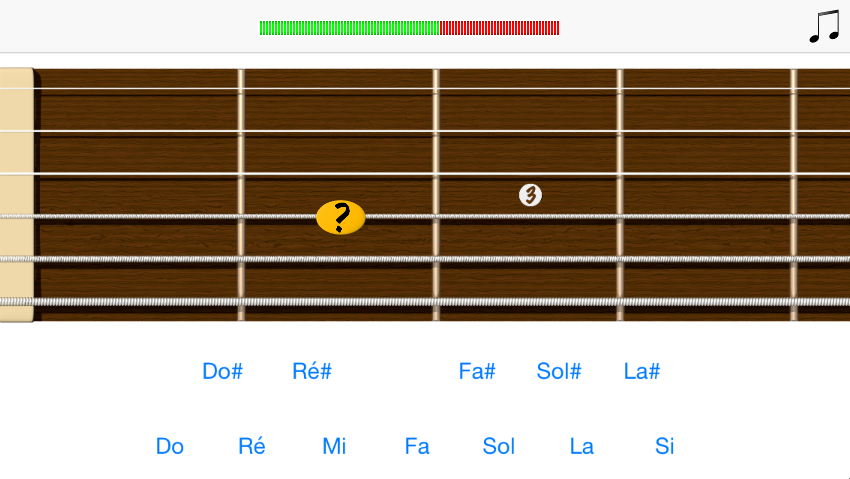
\includegraphics[width=4cm]{images/clavier_question.png}

			\end{column}

			 \begin{column}{0.4\textwidth}

				
			\end{column}

		\end{columns} 

	\end{frame}

	\begin{frame}

   		\frametitle{Manche/clavier}

       		\framesubtitle{Scénario 3}

		\begin{columns}

			 \begin{column}{0.4\textwidth}

				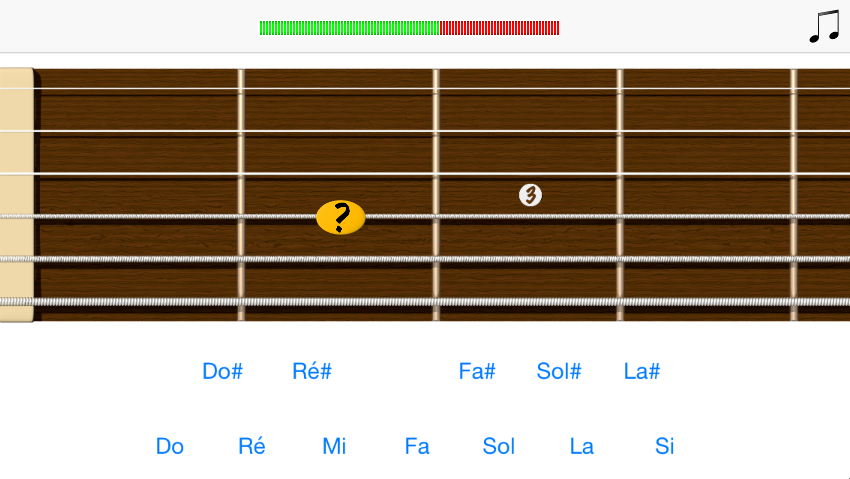
\includegraphics[width=4cm]{images/clavier_question.png}

			\end{column}

			 \begin{column}{0.4\textwidth}

				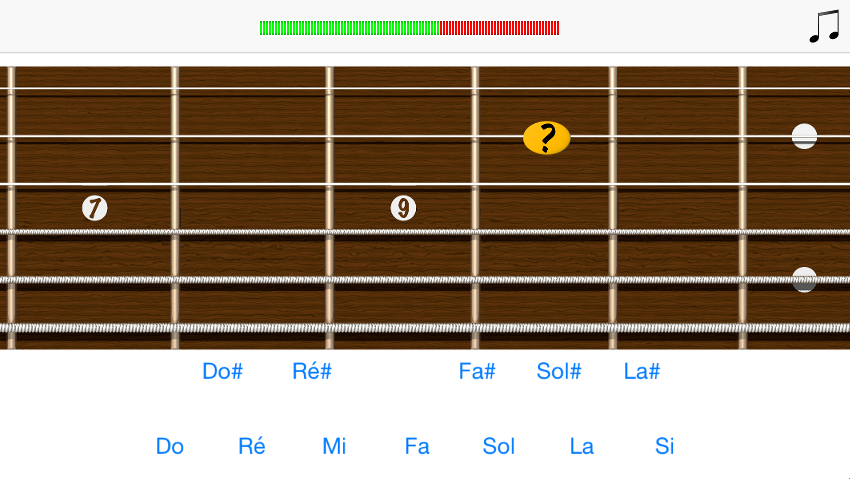
\includegraphics[width=4cm]{images/clavier_question_manche_decale.png}

				
			\end{column}


		\end{columns} 

	\end{frame}

				%****** Scénario 4 ******%


	\begin{frame}

   		\frametitle{Manche/clavier}

       		\framesubtitle{Scénario 4}

		\begin{columns}

			 \begin{column}{0.4\textwidth}

				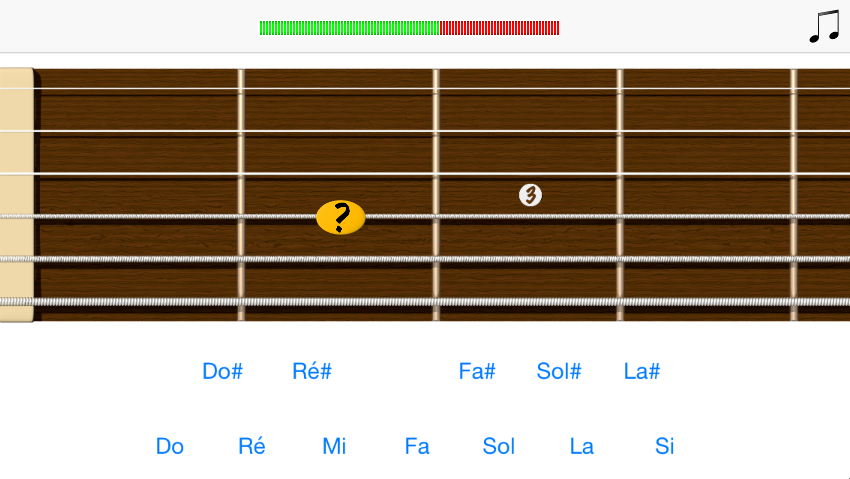
\includegraphics[width=4cm]{images/clavier_question.png}

			\end{column}

			 \begin{column}{0.4\textwidth}

				
			\end{column}

		\end{columns} 

	\end{frame}

	\begin{frame}

   		\frametitle{Manche/clavier}

       		\framesubtitle{Scénario 4}

		\begin{columns}

			 \begin{column}{0.4\textwidth}

				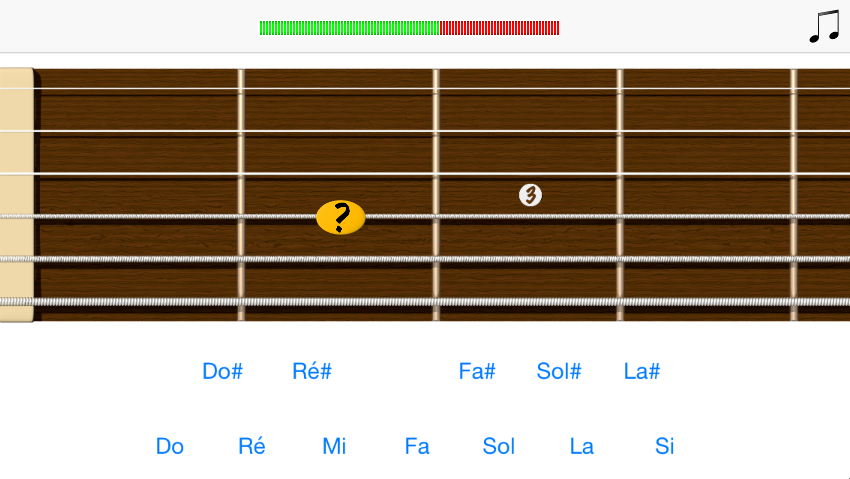
\includegraphics[width=4cm]{images/clavier_question.png}

			\end{column}

			 \begin{column}{0.4\textwidth}

				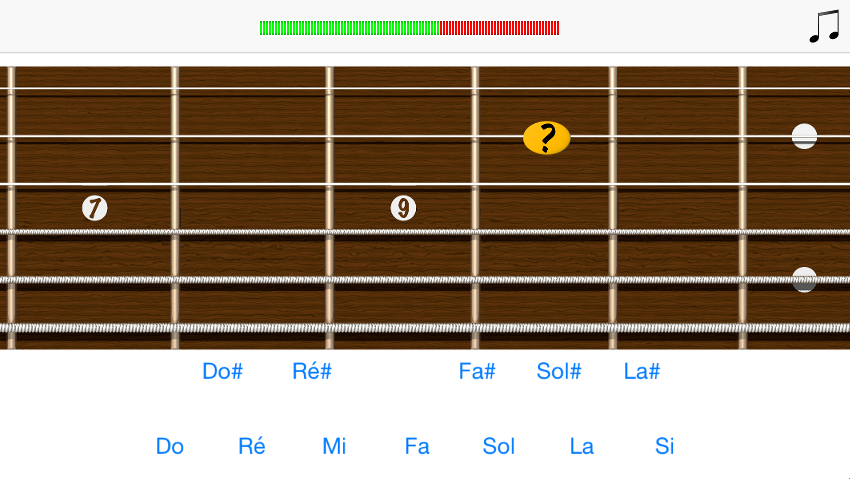
\includegraphics[width=4cm]{images/clavier_question_manche_decale.png}

				
			\end{column}


		\end{columns} 

	\end{frame}





% ******************* Portée/manche *******************

	\subsection{Scénarios portée/manche}

\begin{frame}

   		\frametitle{Portée/manche}

       		\framesubtitle{Scénario 1}

		\begin{columns}

			 \begin{column}{0.33\textwidth}

				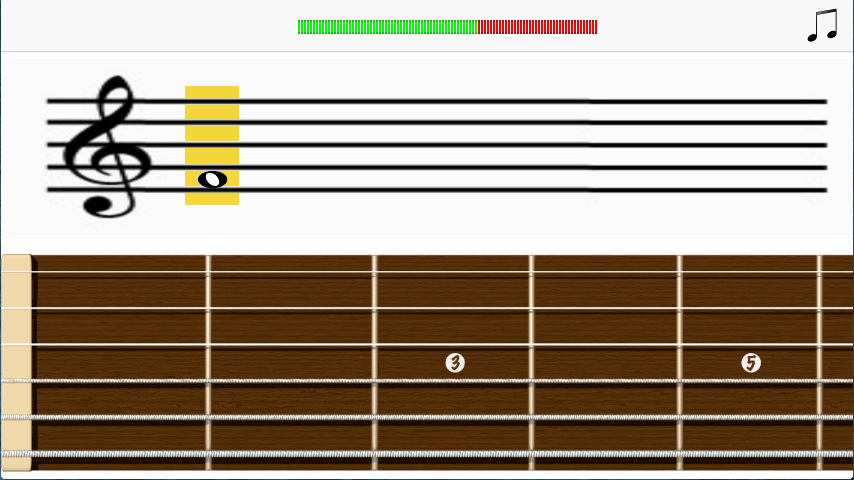
\includegraphics[width=3.5cm]{images/portee_question.png}

			\end{column}

			 \begin{column}{0.33\textwidth}

				
			\end{column}

			 \begin{column}{0.33\textwidth}

				
			\end{column}

		\end{columns} 

	\end{frame}

	\begin{frame}

   		\frametitle{Portée/manche}

       		\framesubtitle{Scénario 1}

		\begin{columns}

			 \begin{column}{0.33\textwidth}

				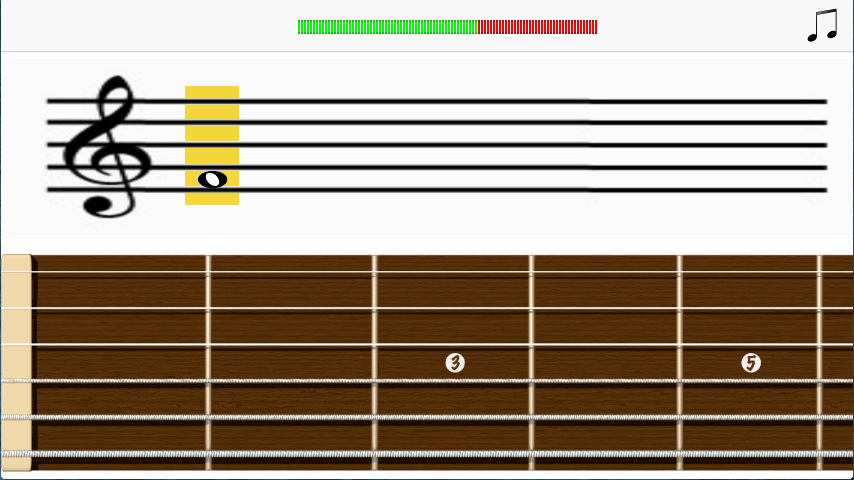
\includegraphics[width=3.5cm]{images/portee_question.png}

			\end{column}

			 \begin{column}{0.33\textwidth}

				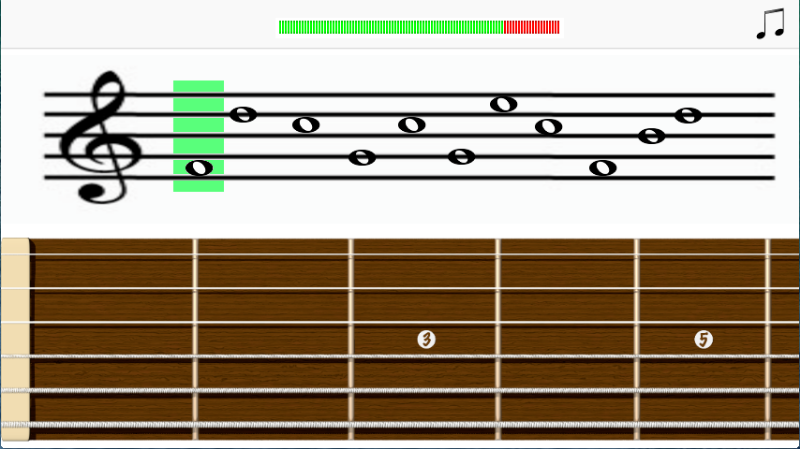
\includegraphics[width=3.5cm]{images/portee_bonne.png}

				
			\end{column}

			 \begin{column}{0.33\textwidth}

				
			\end{column}

		\end{columns} 

	\end{frame}


	\begin{frame}

   		\frametitle{Portée/manche}

       		\framesubtitle{Scénario 1}

	\begin{columns}

	 	\begin{column}{0.33\textwidth}

		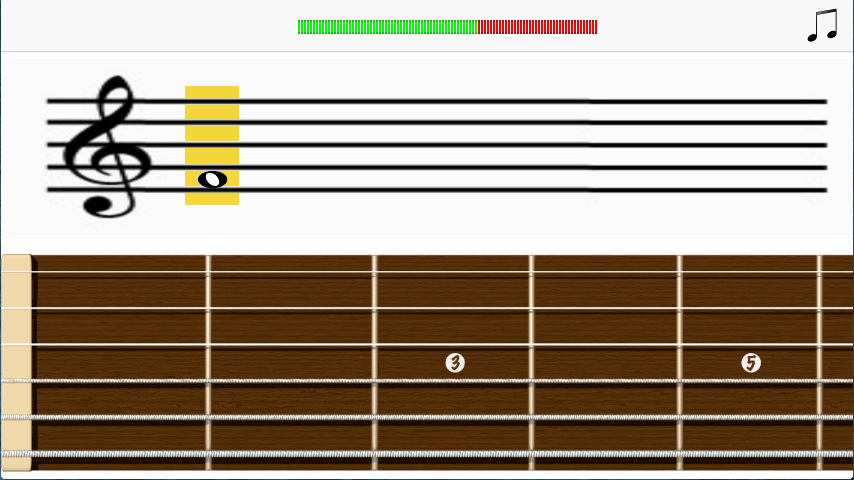
\includegraphics[width=3.5cm]{images/portee_question.png}

		\end{column}

	 \begin{column}{0.33\textwidth}

		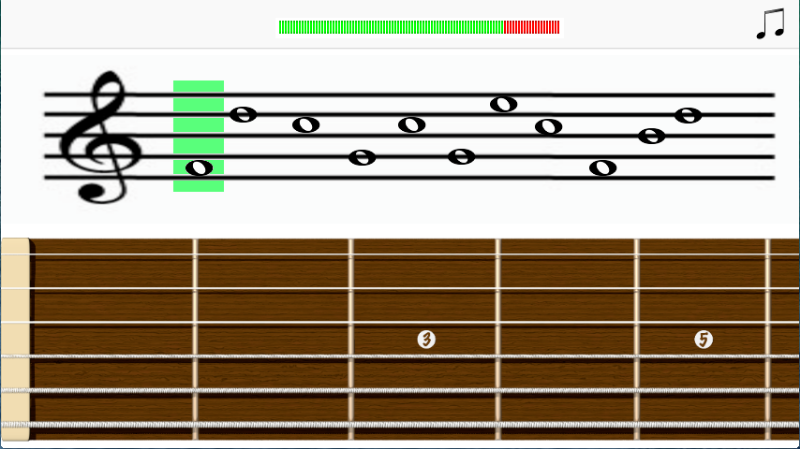
\includegraphics[width=3.5cm]{images/portee_bonne.png}

	\end{column}

	 \begin{column}{0.33\textwidth}

		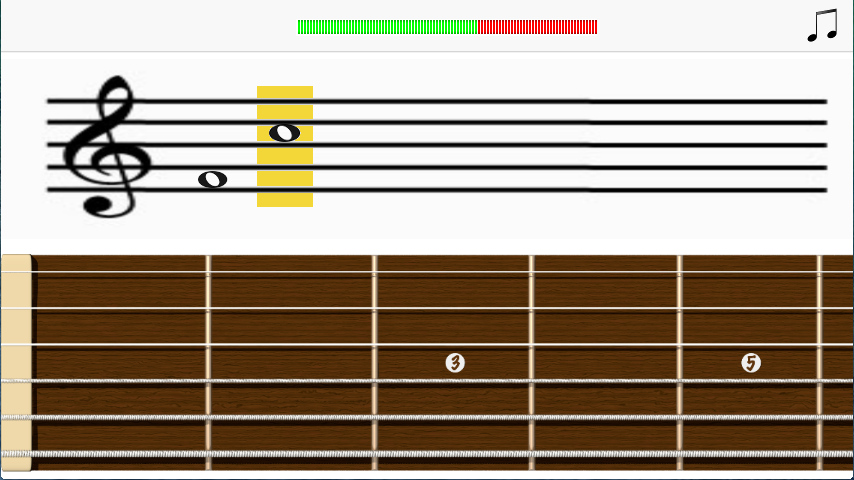
\includegraphics[width=3.5cm]{images/portee_question_2.png}

	\end{column}

	\end{columns} 

	\end{frame}
 


					%** Scenario 2 **%

	\begin{frame}

   		\frametitle{Portée/manche}

       		\framesubtitle{Scénario 2}

		\begin{columns}

			 \begin{column}{0.33\textwidth}

				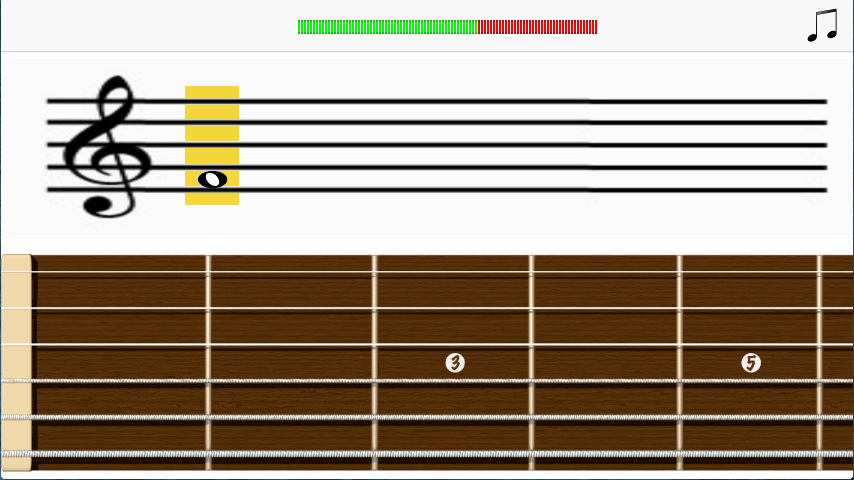
\includegraphics[width=3.5cm]{images/portee_question.png}

			\end{column}

			 \begin{column}{0.33\textwidth}

				
			\end{column}

			 \begin{column}{0.33\textwidth}

				
			\end{column}

		\end{columns} 

	\end{frame}

	\begin{frame}

   		\frametitle{Portée/manche}

       		\framesubtitle{Scénario 2}

		\begin{columns}

			 \begin{column}{0.33\textwidth}

				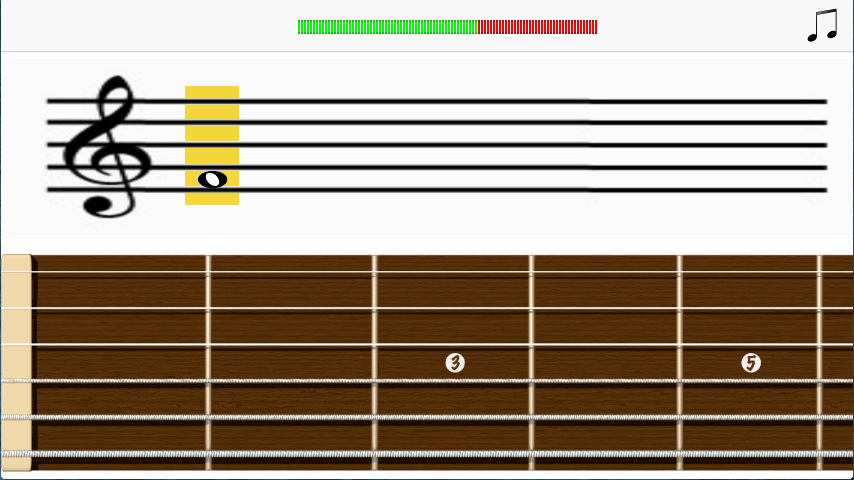
\includegraphics[width=3.5cm]{images/portee_question.png}

			\end{column}

			 \begin{column}{0.33\textwidth}

				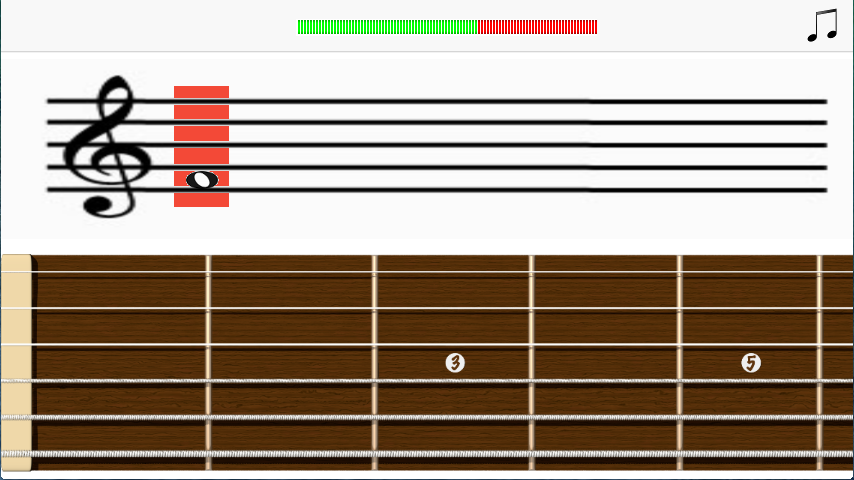
\includegraphics[width=3.5cm]{images/portee_mauvaise.png}

				
			\end{column}

			 \begin{column}{0.33\textwidth}

				
			\end{column}

		\end{columns} 

	\end{frame}


	\begin{frame}

   		\frametitle{Portée/manche}

       		\framesubtitle{Scénario 2}

	\begin{columns}

	 	\begin{column}{0.33\textwidth}

		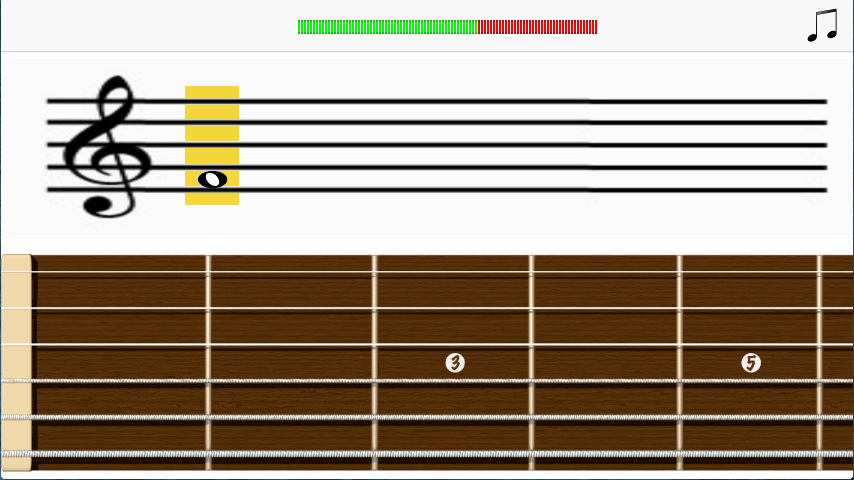
\includegraphics[width=3.5cm]{images/portee_question.png}

		\end{column}

	 \begin{column}{0.33\textwidth}

		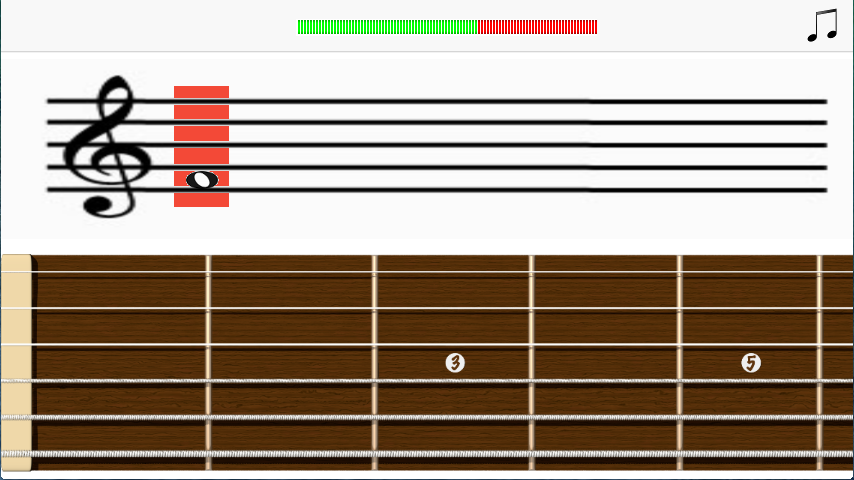
\includegraphics[width=3.5cm]{images/portee_mauvaise.png}

	\end{column}

	 \begin{column}{0.33\textwidth}

		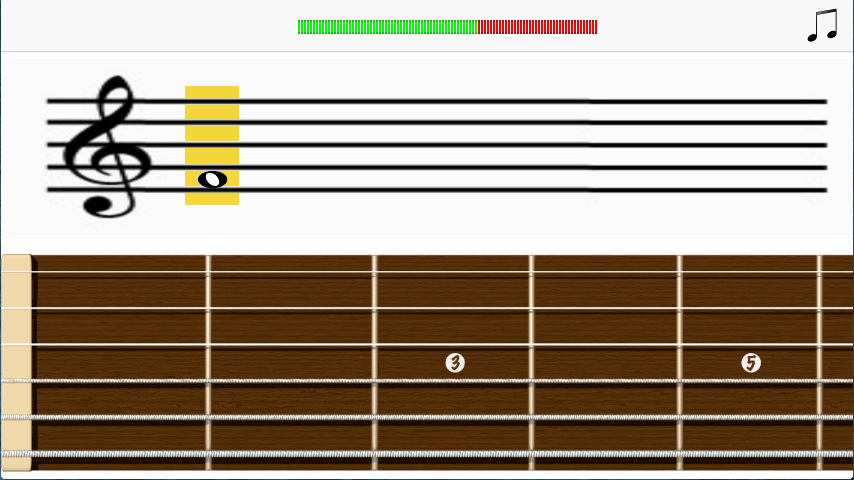
\includegraphics[width=3.5cm]{images/portee_question.png}

	\end{column}

	\end{columns} 

	\end{frame}




				%** Scénario 3 **%


	\begin{frame}

   		\frametitle{Portée/manche}

       		\framesubtitle{Scénario 3}

		\begin{columns}

			 \begin{column}{0.4\textwidth}

				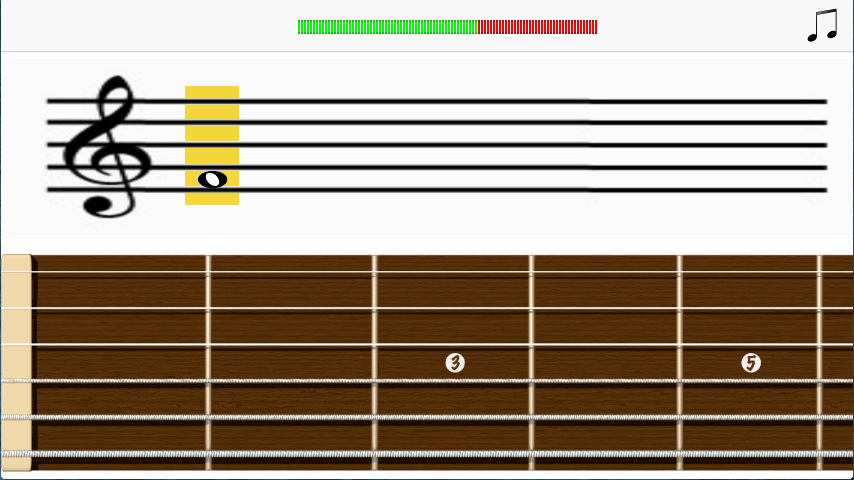
\includegraphics[width=3.5cm]{images/portee_question.png}

			\end{column}

			 \begin{column}{0.4\textwidth}

				
			\end{column}


		\end{columns} 

	\end{frame}

	\begin{frame}

   		\frametitle{Portée/manche}

       		\framesubtitle{Scénario 3}

		\begin{columns}

			 \begin{column}{0.4\textwidth}

				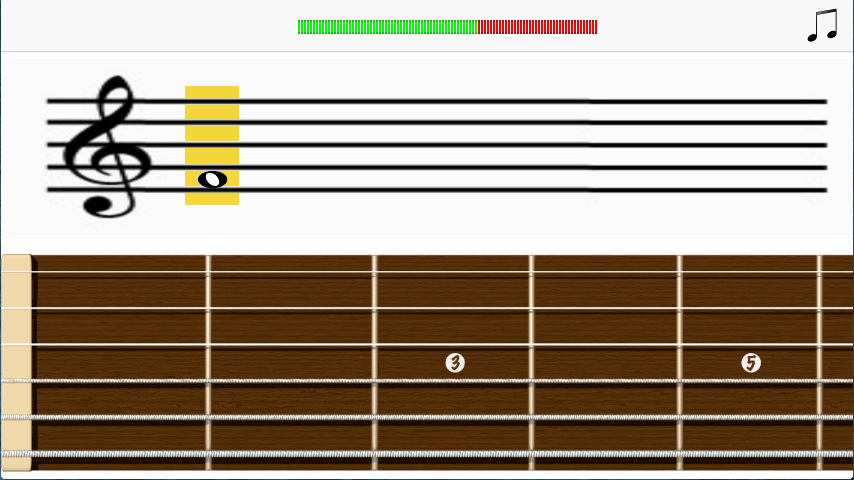
\includegraphics[width=3.5cm]{images/portee_question.png}

			\end{column}

			 \begin{column}{0.4\textwidth}

				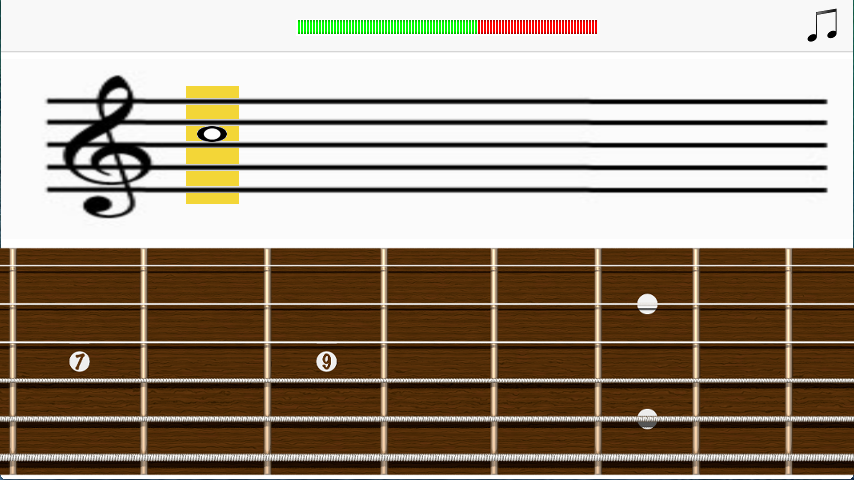
\includegraphics[width=3.5cm]{images/portee_changement_manche.png}

				
			\end{column}


		\end{columns} 

	\end{frame}


	\begin{frame}

   		\frametitle{Portée/manche}

       		\framesubtitle{Scénario 3}

	\begin{columns}

	 	\begin{column}{0.4\textwidth}

		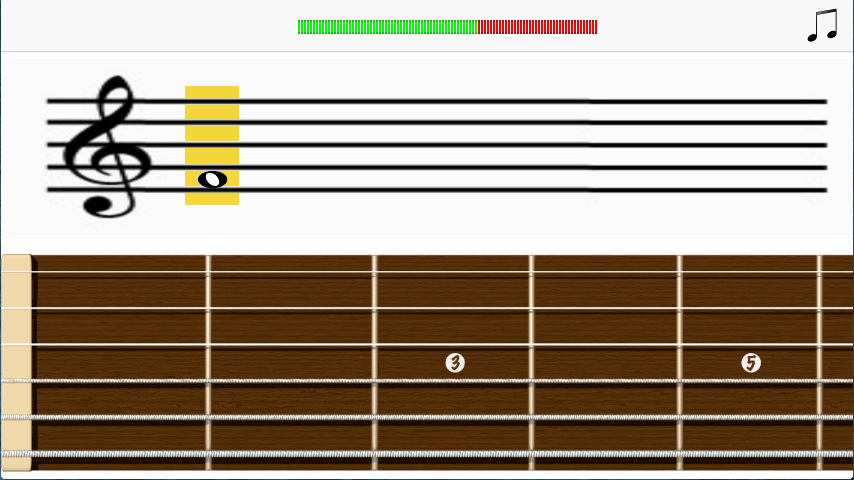
\includegraphics[width=3.5cm]{images/portee_question.png}

		\end{column}

	 \begin{column}{0.4\textwidth}

		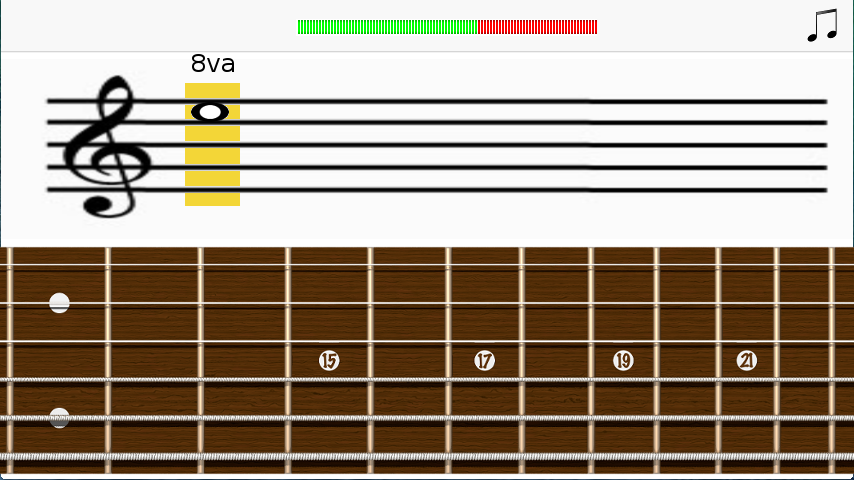
\includegraphics[width=3.5cm]{images/portee_8va.png}

	\end{column}

	\end{columns} 

	\end{frame}



% ***** Implémentation *****

\section{Implémentation}

\subsection{Maquettes}

	\begin{frame}

   		\frametitle{Caractéristiques}


	\begin{itemize}
		\item  Proportion des maquettes 	
		\item  Adaptation dynamique à l'écran
		\item Quatre frettes visibles au démarrage du jeu
	\end{itemize}


	\end{frame}


\end{document}